\chapter{Implementation of Application Energy Monitoring}
\label{chapter:implementation}

\section{Introduction}
The logical design of the Apollo energy estimation calculator was presented in Chapter \ref{chapter:monitoring} and showed how, in principle, we can build a useful energy calculator to fairly allocate energy usage of a collection of host machines, on the basis of the individual application requests processed in a period of time (rather than just the total resource usage of application elements over a period).   Such a calculator can provide a tool for a software architect to understand the energy consumption implications of their architectural decisions and can guide them towards higher energy efficiency for the applications.

The logical design of the calculator is independent of specific technologies and does not specify the details of the implementation, simply the operations that must be performed.  Hence, while it is a type of design, as we are now to implement the calculator it actually acts as our specification and our proof of concept implementation - Apollo - can be implemented in a number of ways using a number of different technology choices and detailed design decisions.

In this chapter we explain how we went about the task of implementing our proof-of-concept calculator, the problems we set out to solve, the choices we made, some of the problems we had to solve and some of the tradeoffs that were necessary.

\section{Initial Decisions}

In order to move forwards efficiently, we needed to narrow the design space for our problem to allow us to focus on the key decisions specific to the problem we were investigating rather than being distracted by the generic decisions that all software projects need to make.

These basic decisions were as follows:

\begin{itemize}
	\item As mentioned in the previous chapter, We will focus on the domain of \emph{microservice-based information systems}, such as those found in large enterprises, Internet-facing systems and Internet-oriented startup companies.  We will not specifically exclude the approach being used with other architectural styles, but where a design decision is required, we will assume that the approach will be used with a microservice-based system.
	\item We will assume that the primary technology "stack" used to implement the system will be \emph{enterprise Java}, meaning software written in Java, running on the JVM, using common open source frameworks and libraries like Spring Boot, Hibernate, Dropwizard, Spring Data, Apache Commons and so on.
	\item We will assume that the primary \emph{execution platform is Linux on Intel}, as this is something of a defacto standard for running large-scale enterprise Java systems.  Where it is possible we will try to make the approach execution platform agnostic (in particular to allow for Windows, another common server execution platform in the enterprise) but again, where a decision needs to be made, we will assume a Linux on Intel host.
\end{itemize}

All of these decisions align us with mainstream industry practice and provide practical options for applying our approach to industrial systems, while narrowing our design decisions to those related to our research problem, rather than generic concerns.

\section{Tracing Application Execution}

Our aim is to provide the application architect with insight into the energy consumption implications of their design decisions, and so simply measuring the energy of the infrastructure hosting the application does not provide enough information for this purpose.  The architect needs to understand the energy implications of the execution of different parts of their application, and most importantly, the energy consumption of certain types of workload.  This will allow them to understand the energy intensive parts of their application and workload and focus on improving the energy characteristics of these application elements.  Comparing the energy characteristics of different elements and workloads will also allow them to see the implications of particular design choices.

This requirement means that we need some way of tracing the execution of workload through the application to produce data equivalent to the traces and spans that we saw in Chapter \ref{chapter:monitoring}.  We considered a number of ways of achieving this.

\emph{Application specific tracing} could be provided by an application as part of its implementation and write special purpose log files or database entries to record how an application request is processed through the application's elements.  While straightforward from our perspective, this is a complex and potentially time consuming feature to add to an application and would be quite complicated to add to an existing system.  We think that this approach would be unlikely to be adopted in practice.

\emph{Application Performance Management} (APM) tools, such as AppDynamics, New Relic and Dynatrace \cite{appdynamics2018, newrelic2018, dynatrace2018} already perform application request tracing to allow them to measure and estimate application performance characteristics.  Initially using a tool like this as the basis of our approach was our preferred option.  In practice though, while attractive to practitioners who were already using the particular tool we would choose, it is a significant barrier to everyone else due to the cost and complexity of deploying these tools.  While we see our work as a potential extension of APM tools, perhaps providing them with a new dimension to their facilities, we decided against basing our approach on one of them.

\emph{Microservice tracing systems} like the open source Zipkin and Jaeger \cite{zipkin2018, jaeger2018} projects were a third alternative that we considered.  These systems are used by application developers to provide standardised trace data about the execution of their applications and provide collection and analysis infrastructure to allow the trace data to be easily used.  When we initially investigated them, they appeared to solve part of the problem of implementing application specific tracing, but still left the application developer with significant work to do.  As we investigated these open source products further we found that they are supported by or integrated into many commonly used application frameworks (for example Zipkin is already integrated into libraries for about 10 languages, including Java, Python, C\# and JavaScript, and just considering Java, it is integrated into more than 15 well known application frameworks including Spring Boot, Dropwizard, Google RPC, Apache HTTP Client and Jersey).  If using a pre-integrated framework, using these tracing systems is very straightforward from an application developer's perspective and normally simply involves starting the data server to receive the trace data and setting some configuration parameters in the framework configuration.

After some experimentation we found that the Zipkin tracing system worked very well for a set of Java microservices and its database was easy to query to extract the trace information we needed.  We concluded that the reliability, easy availability, low implementation overhead, ease of use and large number of existing integrations with widely used application frameworks made Zipkin a good choice for our work.

\section{Estimating Resource Usage of Application Workload}

Once we can reliably trace execution of application requests through the application elements involved in processing them, we can move to considering how to estimate the resource usage of those application elements in order to work out the resource consumption of the requests processed by the application.  The key requirement here is to be able to collect reliable samples of the resource usage of the application elements on a very frequent and predictable basis (e.g. every couple of seconds).  Ideally the samples will be in terms of cumulative usage rather than usage at that point in time, as these are much easier to use for our purposes.

The only practical source of application resource usage statistics is the application execution platform.  There are a number of sources of statistics that we could use, each with slightly different characteristics.

The simplest option is to use \emph{native operating system tools} such as \texttt{sar} and \texttt{pidstat} on Linux and \texttt{procmon} and \texttt{perfmon} on Windows.  In principle these tools can collect resource usage statistics for application processes on the machine.  However in practice, our industrial experience and recent investigation for this work, suggests that they are really intended for collecting host-level statistics or for interactive investigation of a performance problem on a machine, by a skilled administrator.  They do not provide an easy way to get a reliable stream of samples of cumulative usage over time written into an accessible form.

An alternative is to bypass the tools and access the \emph{operating system performance counters} directly.  Like most modern operating systems, Windows and Linux both implement a set of performance counters in their kernels, which are used for monitoring performance and throughput of workload executed by the machine.  These counters are used by the operating system tools to provide the data they need to operate and so by accessing the counters directly, we can avoid any limitations in the tools and still achieve consistent results.  Linux provides access to its performance counters via the very convenient \texttt{{/proc}} file system, which exposes all of the kernel's counters for global and process-specific metrics, via a pseudo file system interface (which can be read using standard text processing tools or through the standard file system API).  Windows provides access to its performance counters via the \texttt{perfmon} tool or through an API which is accessible via PowerShell (the modern Windows scripting language) or a conventional programming language.  In principle we can build any collection tool we want using these interfaces or we can use metrics collection servers such as \texttt{telegraf} or \texttt{collectd} \cite{telegraf2018, collectd2018} to read them automatically and store them in a suitable database for us.  During initial research, this approach was our preferred option, however in practice we found it quite difficult to get a usable set of statistics for our application.  The main problem we faced was that the collector does not know which workload on the machine belongs to a particular application.  Therefore we had to collect everything at operating system process level, which potentially generates huge amounts of unnecessary data.  We also found that the business of building a reliable collector was more difficult than initially assumed and that linking the trace data to the dataset we could collect easily from operating system counters was quite difficult to do reliably.  These difficulties were not insurmountable, but led us to consider whether there were other options we could consider.

The third option we investigated was to use \emph{Docker} \cite{docker2018} as a packaging technology for the application elements and to allow us to collect resource usage statistics.  Docker is an operating system virtualisation technology which uses operating system mechanisms (such as "cgroups" and "kernel namespaces" on Linux) to isolate processes from each other, providing the illusion that each is running on a separate machine.  Docker also provides a packaging convention that allows software to be packaged into reusable packages called "images" which are combined at runtime to form runtime environment known as a "container".  Docker also provides a set of management APIs and tools to allow containers to be interrogated, managed and controlled.  Docker is rapidly becoming a de-facto standard in the industry to package, deploy and manage microservices both on general host computers (where Docker becomes an execution environment on top of the operating system) and more abstract, container based platforms like Kubernetes \cite{kubernetes2018} where Docker forms part of a sophisticated platform providing demanding quality properties like scalability and resilience, across a cluster of host computers.

Our interest in Docker lies in its ability to provide a low-overhead, isolated environment for running application elements (in our case, microservices specifically).  If we can assume that all of the microservices within our system are packaged and then run as Docker containers then it provides us with the ability to extract accurage resource utilisation statistics for the microservice running in the container.  Another benefit of using Docker is that each container has its own network (IP) address which can be found via the runtime metadata available via Docker's management API.  This greatly simplifies the process of relating the resource usage data to the request traces from Zipkin as the network address is a shared piece of information between the two.

We believe that requiring application elements (the microservices) to be packaged and run as Docker containers is realistic and reasonable, given its wide and growing adoption in industry, particulary for microservice-based systems.  Therefore this combination of factors resulted in us deciding to use Docker as the basis for collecting application resource utilisation statistics.

The second part of collecting utilisation statistics is how they are extracted and stored from the execution platform.  In our case, our experimentation with Docker quickly revealed that a number of open source projects, including \emph{cAdvisor} \cite{cadvisor2018} and \emph{Telegaf} \cite{telegraf2018}, provide close integration with Docker and can extract and store the utilisation statistics data in different database systems.

After some experimentation we chose to use Docker with Telegraf, storing utilisation statistics in the \emph{InfluxDB} \cite{influxdb2018} open source time-series database to provide us with reliable application element resource utilisation statistics gathering.

\section{Estimating Resource Usage of the Host Platform}

Estimating resource usage of the underlying host platform is simpler than gathering the same information for the application elements, as host-level statistics gathering is a mature and widely used technology, provided by all major operating system platforms.

In our case we need to achieve reliable resource utilisation sampling of the host platform - the underlying Linux operating system - and have them stored in a database that allows us to extract them through a query interface to support the calculation process.  Ideally if the statistics are in a similar form to the statistics for the application level resource utilisation (e.g. the same timestamp convention and data types used), then this is likely to make the implementation of the calculator easier.

Our earlier investigation of the \emph{Telegraf} data collection server to extract and store application-level utilisation statistics revealed that it can be configured to extract and store host-level utilisation statistics too, and that this facility is provided as part of the standard distribution of the (open source) product.  When we tested the host resource utilisation statistics feature of Telegraf we found that it was straightforward to use and reliably stored accurate statistics in the same database as the application-level statistics.  The host-level statistics used the same basic conventions as the application-level statistics (e.g. they were both cumulative utilisation statistics using the same timestamp conventions).

Therefore we were able to solve the host-level resource utilisation statistics gathering problem by simply extending the configuration of the Telegraf server and the extension of the data set it stored to include host-level statistics.

\section{Estimating Energy Usage of the Host Platform}

As explained when we discussed the motivation for this work in Chapter \ref{chapter:introduction} the field of energy estimation is relatively young and reliable approaches for energy estimation of individual devices and applications are only just emerging.  Our work does not intend to address the problem of estimating energy consumption for a single host computer, but rather requires a reliable energy consumption metric to be available.

As explained in Chapter \ref{chapter:monitoring} there are two main approaches available to us that can provide energy usage of our underlying host platform, physical energy consumption metrics made available via a DCIM platform and model-based energy consumption estimation using machine utilisation levels and published benchmark results.

In many industrial situations, a DCIM platform will be available and energy consumption metrics for all or a subset of host machines will be available through it.  However in our research environment we did not have access to such a platform and in many industrial situations this will be the case too.  While the state-of-the-art in organisation design is to integrate development and operations groups, they are frequently still separate and so even when a DCIM platform is available, software architects may well not be able to access it easily.

Therefore we decided to use a model-based approach to estimate the energy consumption of the host, but to ensure that it was easily replaceable with alternative models or with queries to a DCIM platform if one was available.

The approach used to estimate the energy usage of a host was explained in section \ref{subsection:calculation-specification} and relies upon published power consumption benchmark results associated with the \cite{lange2009-specpower} benchmarks.  An example data set for power consumption for a specific model of server host is shown in \ref{table:powervalues}

\begin{table}
\centering
\caption{SPECPower 2008 Benchmark Results for \\Dell PowerEdge R730 (Intel Xeon E5-2699 v4 2.20 GHz)}
\label{table:powervalues}
\footnotesize
\begin{tabular}{|c|c|c|}
\hline
Machine Load & Power Consumption (W) & W / \% \\
\hline
\hline
Active Idle  &  44.6 & -    \\
10\%         &  84.8 & 8.48 \\
20\%         & 102.0 & 5.10 \\
30\%         & 120.0 & 4.00 \\
40\%         & 136.0 & 3.40 \\
50\%         & 150.0 & 3.33 \\
60\%         & 163.0 & 2.64 \\
70\%         & 181.0 & 2.58 \\
80\%         & 205.0 & 2.56 \\
90\%         & 238.0 & 2.64 \\
100\%        & 272.0 & 2.72 \\
\hline
\end{tabular}
\end{table}

We use this style of benchmark data combined with the machine type executing our application workload and the utilisation level metrics of the server executing the load to estimate total server energy consumption at a particular point in time, as explained in section \ref{subsection:calculation-specification}.

We have also added a derived column to show the power consumption per percentage point of server utilisation at each level of utilisation.  This clearly illustrates the need to keep servers busy from an energy efficiency perspective as it an be clearly seen that 1\% utilisation when the machine is quiet is three times more expensive in energy consumption terms than 1\% utilisation when the machine is busy.

\section{Implementing the Calculator}

\subsection{Architecture of the Calculator}

The implementation design of the system is shown in the simple block diagram in Figure 3. The system elements filled with the fine dotted pattern are the elements of the application (Application Services, Black-Box Services and Asynchronout Processors), the system elements filled with the fine cross-hatching are data elements, while the Apollo Energy Estimator is filled with the light solid fill.  The unshaded elements are third party technologies which are reused unchanged as part of the implementation.

\begin{figure}
\centering
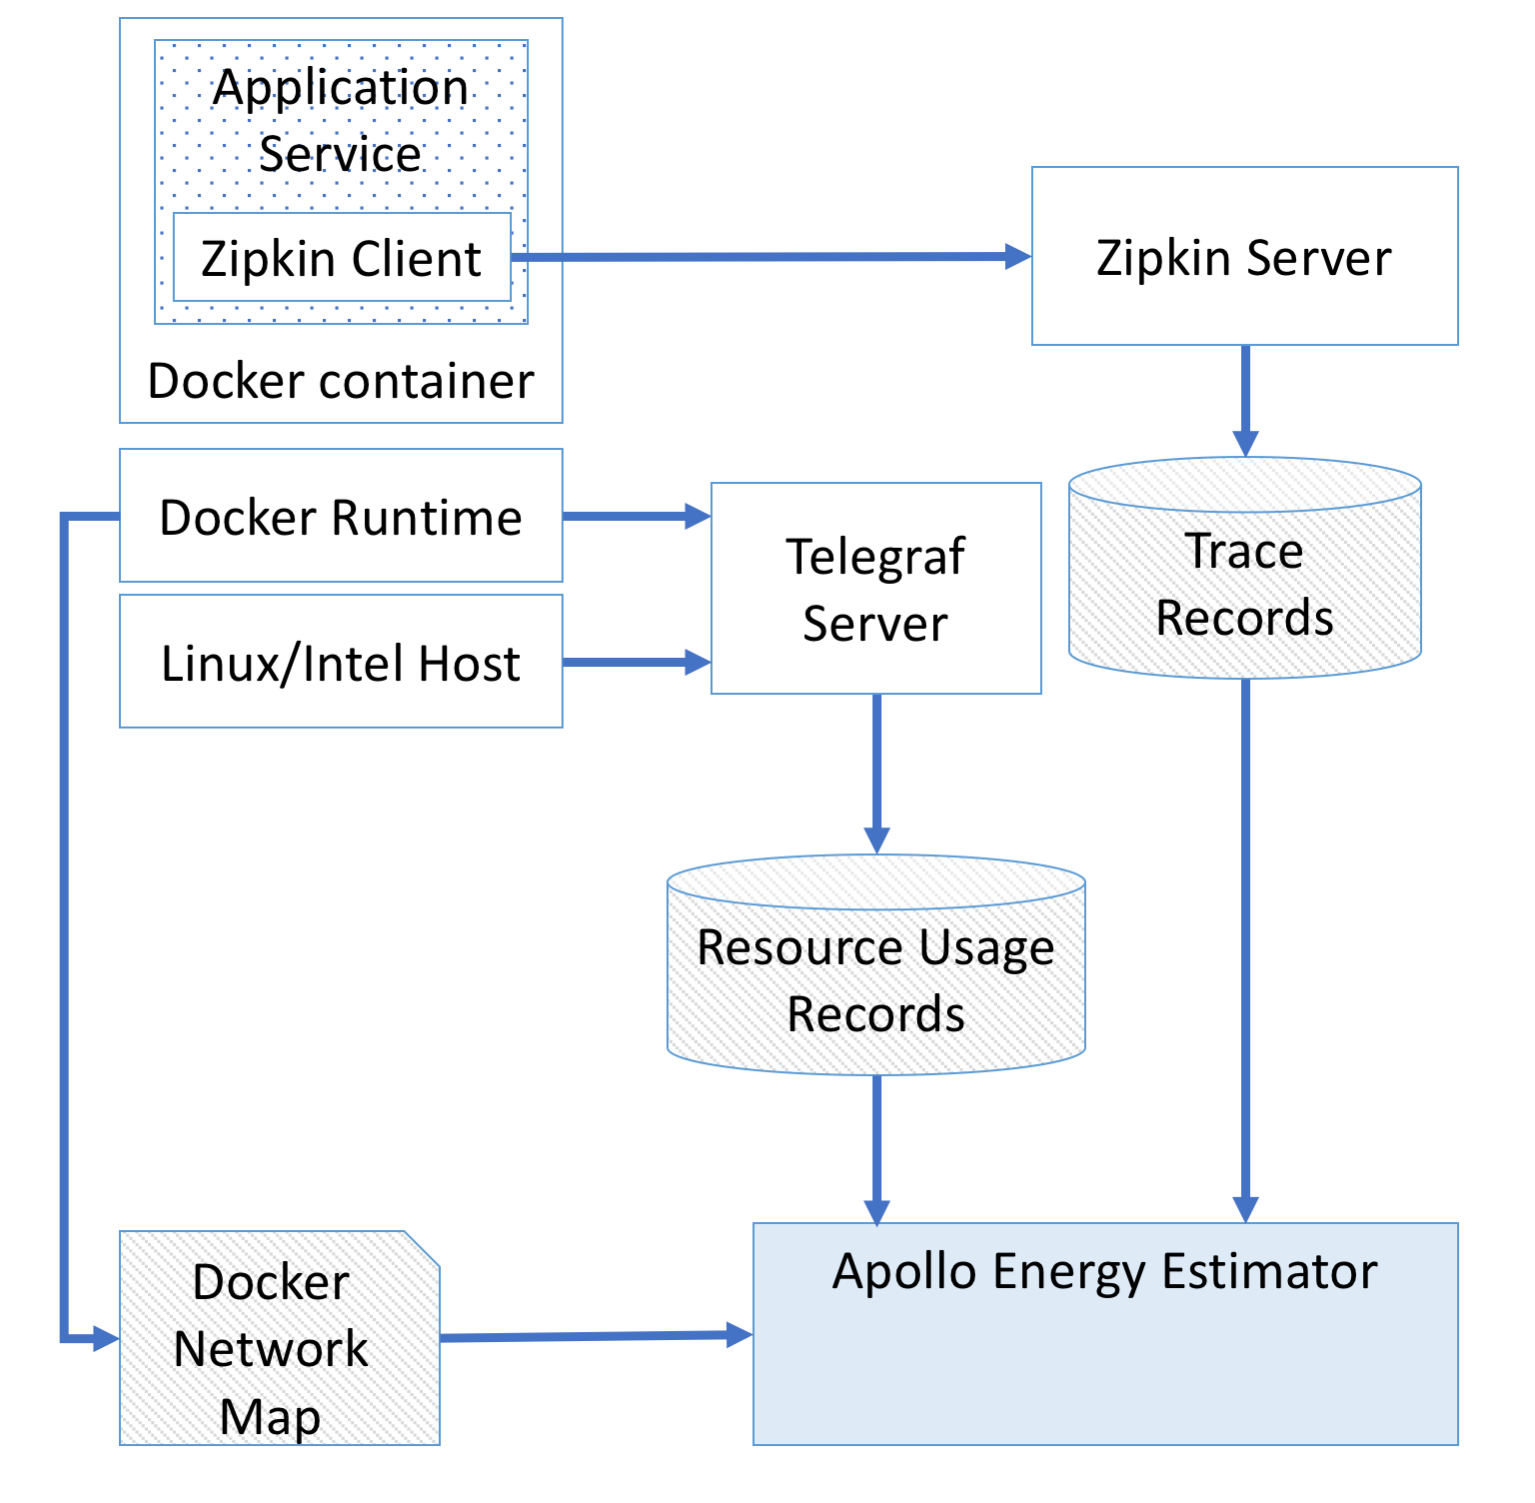
\includegraphics[width=0.5\textwidth]{Figures/implementation-design}
\caption{Implementation of the Apollo Energy Estimator}
\label{figure:implementation}
\end{figure}

The significant third-party technologies used in this implementation are:
\begin{itemize}
\item Docker - as mentioned above, all application elements need to run within Docker containers.  This allows metadata about the elements to be retrieved and resource usage statistics to be gathered.
\item Zipkin - a trace of the invocations to and between application elements is required and as explained above, the Zipkin tracing system is used to achieve this.
\item Telegraf - the Docker platform produces a stream of resource usage statistics for the containers that it is executing.  The Telegraf agent collects these metrics and stores them in a timeseries database for easy retrieval.
\item InfluxDB - is used as the timeseries database for the Resource Usage Records.
\end{itemize}

TODO

\subsection{The Software Structure}

TODO




\subsection{The Calculation Algorithm}

TODO

\section{Limitations of the Calculator}

The design described in this paper has been validated via proof-of-concept implementations of each of its significant decisions and mechanisms, but not yet built.  Therefore the next step in the work is a full, robust implementation which can be utilised and validated to create a useful energy estimation mechanism.
The design described here is the first development of the ideas and has a number of limitations, which can be addressed in future work.

Our approach estimates energy usage for individual requests, by estimating the energy usage of each container as the request is processed.  This allows some degree of isolation as other workload which does not use these containers can be running in the application without it distorting the results.  For Application Service elements this is useful, as they are usually replicated for scalability reasons and so workload can run in the replicas that are not processing the request of interest.  However, care must be taken not to have workload running through shared services (such as databases) which would distort the energy estimation.  This is a limitation of the current version of the design. In practice, we believe that architects are likely to expect this constraint, as it is similar to the situation for other non-functional tests like performance and scalability.

The use of the architectural description data is somewhat unsatisfying as the rest of the inputs to the process are automatically generated.  The creation of the architectural description is a burden for the architect and could be performed incorrectly.  A more sophisticated tracing system, which can trace the activity of “black box” components could go some way to addressing this and could potentially be achieved by lower-level tracing in the operating system and network layer.

The system does not provide the architect with any visualisation or analytics view of the data in order to help draw insights from it.  While not the focus of this work, there are a number of well-known tools (such as Graphana) that could be used to create a visual interface for understanding the results of the analysis.

Third, the energy estimates for each trace and span are derived from sampled resource usage statistics for the corresponding container.  The sample times will very rarely align with the start and end times of the traces and spans and so estimates will need to be made, based on the samples available.  Depending on the sampling interval of the resource monitoring and the timing of the traces and spans, it is possible that the simple estimation approach we use could prove to be inaccurate (perhaps missing peaks and troughs between sample intervals).  The sample intervals we achieve in practice are short (TODO - HOW LONG?) and so we do not believe that this is a significant limitation, but does need to be monitored in practice.

\section{Summary}

TODO

\textit{Possibly useful text after this point to reuse ...}



The operation of the energy estimation system is similar to the simpler functional design explained earlier.  The elements of the system and the responsibilities of each and their key interactions are as follows:

\begin{itemize}
\item Application Service - represents the regular microservices that comprise the application under investigation.  The implementation of these services are under the control of the development team and they have the responsibility to generate Zipkin trace records (via the Zipkin Client library) to record their activity (although this will usually be achieved automatically through use of an application framework like Spring Boot).
\item Other Service - represents the services within the system which cannot be altered by the development team (“Blackbox Services”) or services which, although part of the system, do not take a direct part in request processing but are triggered as a side effect of it (“Asynchronous Processors”).  These system elements do not generate Zipkin traces.
\item Docker Container - the runtime container for all of the application system elements.   It provides isolation for the element within it and an interface to the Docker Runtime.
\item Docker Runtime - is the execution platform for the application system elements, through their use of containers.  The Docker Runtime is responsible for maintaining the topology of the Docker environment (e.g. which containers are running) and tracking resource utilisation of each container (CPU, memory, disk i/o and network i/o).  It streams the container level resource utilisation metrics to the Telegraf Server.
\item Zipkin Client - a client programming library used by Application Services to generate trace records and forward them to the Zipkin Server for storage.  The application code may invoke this library directly or it may be invoked automatically by an application framework like Spring Boot or Drop Wizard.
\item Zipkin Server - accepts incoming streams of trace records from application elements, stores them in the Trace Records database, and provides access to the records (although the records can also be accessed directly from the database, which is what we do in this case).
\item Trace Records - the database of trace records from Zipkin, recording application element activity.
Telegraf Server - an open source metrics collection agent, which accepts the stream of resource usage metrics from Docker and writes them to the Resource Usage Records database.
\item Resource Usage Records - a database of container level resource usage metrics, originally generated by the Docker Runtime.  This is ideally a timeseries database (we use InfluxDB) to allow efficient storage and retrieval of traces and spans by time range.
\item Docker Network Map - the Docker part of the system identifies architectural elements by container ID (which are large numbers) whereas the Zipkin part of the system has no visibility of container IDs and identifies architectural elements primarily by network address.  The Docker Network Map is a datastructure allowing a mapping between the two worlds, and is generated using the Docker “network inspect” command or API call.
\item xADL Architectural Description - as explained previously, in order to make a good estimation of energy usage, we need to be able to understand all of the architectural elements involved in a request.  Some form of machine readable architectural description is needed to provide this information and we have selected xADL as the notation for this, given its relative maturity, standard XML-based technology and tools.
\end{itemize}

Apollo Energy Estimator - is the calculator that produces the energy estimate for each request made to the system.  This architectural element implements the algorithm defined in Figure \ref{figure:implementation}. This means that it:

\begin{itemize}
\item Reads the Trace Records store to extract the Zipkin traces and spans.
\item For each trace that it finds, uses the Network Map to identify the containers that correspond to each trace and span that produced the traces and spans.
\item Reads the xADL Architectural Description to identify the other containers which the architect wishes to be included in the energy estimate for particular requests (based on the containers involved in processing each trace and the relationships between those containers and other containers found in the architectural description).
\item Using the container identities and the start and end times of the corresponding trace or span records, reads the Resource Usage Records store to find the CPU, memory and IO consumption of each container during the relevant time period. 
\item Sums the resource usage statistics for each trace and its child spans to produce total resource usage per request.
\item Calls the energy model to estimate energy usage for the resource usage for each request.
\end{itemize}

The result of this set of element interactions will be the Energy Estimator producing a set of energy consumption estimates for each of the trace records that it finds in the Trace Records store when it is run.

